\documentclass[paper=a4, english, ngerman, romanian]{scrartcl}

\usepackage[a4paper,left=2cm,right=2cm,top=2.5cm,bottom=3cm]{geometry}
\usepackage[ngerman]{babel}
\usepackage{tabularx}
\usepackage[utf8]{inputenc}
\usepackage{multirow}
\usepackage{listings}
\usepackage{graphicx}
\usepackage[absolute]{textpos}
\usepackage{amsmath}
\usepackage{mathtools}
\usepackage{amssymb}
\usepackage{dsfont}
\usepackage{wasysym}
\usepackage{enumitem}
\usepackage{stmaryrd}

\parindent 0pt
\lstset{basicstyle={\ttfamily\scriptsize}, tabsize=4}
\begin{document}

\begin{titlepage}
	\title{Datenbanksysteme SS17: Projekt\\ 3. Iteration}	
	\subtitle{Dozentin: Agnes Voisard}
	\author{Bernadeta Chișărău, Dor Cohen, Mihai Renea}
	\date{\normalsize \today}
\end{titlepage}

\maketitle								% Erstellt das Titelblatt
\vspace*{-8cm}							% rückt Logo an den oberen Seitenrand
\makebox[\dimexpr\textwidth+1cm][r]{	%rechtsbündig und geht rechts 1cm über Layout hinaus
	
\includegraphics[width=0.4\textwidth]{src/fu_logo} % fügt FU-Logo ein
}

\vspace{7cm}							% Abstand
\rule{\linewidth}{0.8pt}				% horizontale Linie
	\section{Clusteranalyse}
		Für die Clusteranalyse haben wir den K-Means Algorithmus mithilfe der java-ml Library eingesetzt. Der Algorithmus partitioniert die Menge der Hashtags in 6 Clusters, wo jedes Hashtag ein 2-dimensionales Vektor mit den folgenden Metriken ist:
		\begin{itemize}
			\item Hashtag-Wichtigkeit -- als Durchschnitt der Wichtigkeitswerten aller Tweets, die Hashtag $h$ enthalten.\\
			Wichtigkeit $W_T(t)$ eines Tweets $t$:\\
			\begin{equation*}
				W_T(t) = ^4\sqrt{\frac{t_{favorites\ count} + t_{retweet\ count}}{2}}
			\end{equation*}
			Wichtigkeit $W_H(h)$ eines Hashtags h:
			\begin{equation*}
				W_H(h) = \frac{\sum_{t \in T} W_T(t)}{|T|}
			\end{equation*}
			Wo $T$ die Menge der Tweets, die Hashtag $h$ enthalten.
			
			\item Hashtag-Occurence -- wie oft ein Hashtag insgesamt auftaucht.
		\end{itemize}
		
		Anschließend speichern wir die neu-erzeugten Informationen in einer neuen Tabelle, \textit{hashtag}. Damit kann man für die Visualisierung die gebrauchten Werte einfach ablesen. Dadurch entsteht die aktuelle DB-Schema:
		
		\begin{center}
			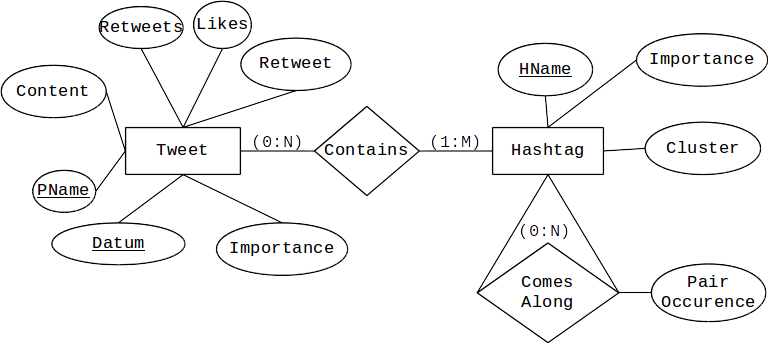
\includegraphics[scale=0.6]{src/MinMax_Diagram}
		\end{center}
		
		\pagebreak

	\section{Datenvisualisierung}
	
		Um die Datenvisualisierung zu vereinfachen haben wir ein Programm geschrieben (Node\_data\_creator.java), das die Informationen aus der Datenbank in JSON-Dateien bereitstellt, und zwar:
			\begin{itemize}
				\item	\textit{plots.json} - Informationen für die Visualisierung des Hashtagnetzwerkes - Knotenpositionen (nodes-Array) und Verbindungen (edges-Array):
				\begin{lstlisting}
{
   "nodes": [
     {
       "color": "rgb(r,g,b)",
       "size": 100,
       "x": "x",
       "y": "y",
       "id": "hname",
       "label": "hname",
       "type": "tweetegy"
     },
     .
     .
     .
   ],
   "edges": [
     {
       "id": "i",
       "source": "hname1",
       "target": "hname2"
     },
     .
     .
     .
    ]
}
				\end{lstlisting}
				
				\item \textit{days.json} - Liste aller Tagen, mit der Anzahl der verschiedenen Hashtags, für die Zeitanalyse:
				
				\begin{lstlisting}
[
   {
     "x": x,
     "y": sum over "htags",
     "label": yy-mm-dd,
     "htags": [
       {
         "y": y1,
         "hname": "hname1"
       },
       {
         "y": y2,
         "hname": "hname2"
       },
       .
       .
       .
     ]
   },
   .
   .
   .
]
				\end{lstlisting}
\newpage
Visualisierung des Hashtagnetzwerkes 

\begin{itemize}
\item haben die Javascript-Bibliothek sigmajs benutzt
\item haben uns bewusst gegen eine kreisförmige Darstellung des Netzwerkes entschieden, weil diese die Lesbarkeit unseres Graphen erheblich erschwert hätte.
\item Stattdessen haben wir uns für eine andere Art der Visualisierung entschieden, die die Visualisierung "in die Breite zieht" und das Problem der sehr ungleichmaessigen Verteilung loest
\item Format unserer Input-Datei: .json
\\
\end{itemize}

Visualisierung der Haeufigkeit 

\begin{itemize}
\item haben die Javascript-Bibliothek d3js benutzt
\item auf der x-Achse tauchen alle im Datensatz aufgelisteten Tage auf vom 5.01.2016 bis zum 27.9.2016
\item Die y-Achse geht von 0 bis 93, wobei 93 die hoechste Anzahl an Hashtags darstellt, die an einem Tag getweetet wurden
\item Da die Darstellung der Tage an der x-Achse aufgrund des großen Datensatzes nicht lesbar war, haben wir mit d3-tip Tooltips eingefügt, sodass wir beim Gleiten über jeden Balken das jeweilige Datum lesen koennen.
\item Format unserer Input-Datei: .json
\item fuer die Darstellung der Haeufigkeit des Auftretens eines auswaehlbaren Hashtags haben wir eine json-Datei mit folgendem Beispieldatensatz benutzt:
\begin{lstlisting}
[
   {
     "x": 0,
     "y": 5,
     "HLabel": "MakeAmericaGreatAgain",
     "DLabel": 2016-01-05
       },
       .
       .
       .
     ]
   },
   .
   .
   .
]
				\end{lstlisting}
 
\end{itemize}
was in diesem Fall bedeutet, dass der Hashtag "MakeAmericaGreatAgain" an dem Tag    2016-01-05, was an 0ter Stelle auf der x-Achse steht, 5 Mal vorgekommen ist.\\



Unser Projekt ist auf GitHub unter diesem Link zu finden: https://github.com/derMihai/DBS_Project

  

			\end{itemize}
	
\end{document}
